\documentclass[a4paper,twoside]{article}
\usepackage{blindtext}  
\usepackage{geometry}

% Chinese support
\usepackage[UTF8, scheme = plain]{ctex}

% Page margin layout
\geometry{left=2.3cm,right=2cm,top=2.5cm,bottom=2.0cm}


\usepackage{listings}
\usepackage{xcolor}
\usepackage{geometry}
\usepackage{amsmath}
\usepackage{float}
\usepackage{hyperref}

\usepackage{graphics}
\usepackage{graphicx}
\usepackage{subcaption}
\usepackage{epsfig}
\usepackage{float}

\usepackage{algorithm}
\usepackage[noend]{algpseudocode}

\usepackage{booktabs}
\usepackage{threeparttable}
\usepackage{longtable}
\usepackage{tikz}
\usepackage{multicol}

% cite package, to clean up citations in the main text. Do not remove.
\usepackage{cite}

\usepackage{color,xcolor}

%% The amssymb package provides various useful mathematical symbols
\usepackage{amssymb}
%% The amsthm package provides extended theorem environments
\usepackage{amsthm}
\usepackage{amsfonts}
\usepackage{enumerate}
\usepackage{enumitem}
\usepackage{listings}
\usepackage{minted}


\usepackage{indentfirst}
\setlength{\parindent}{2em} % Make two letter space in the first paragraph
\usepackage{setspace}
\linespread{1.5} % Line spacing setting
\usepackage{siunitx}
\setlength{\parskip}{0.5em} % Paragraph spacing setting

% \usepackage[contents =22920202204622, scale = 10, color = black, angle = 50, opacity = .10]{background}

\renewcommand{\figurename}{图}
\renewcommand{\listingscaption}{代码}
\renewcommand{\tablename}{表格}
\renewcommand{\contentsname}{目录}
\floatname{algorithm}{算法}

\graphicspath{ {images/} }

%%%%%%%%%%%%%
\newcommand{\StudentNumber}{22920202204622}  % Fill your student number here
\newcommand{\StudentName}{熊恪峥}  % Replace your name here
\newcommand{\PaperTitle}{实验(三)自顶向下的语法分析器}  % Change your paper title here
\newcommand{\PaperType}{编译原理} % Replace the type of your report here
\newcommand{\Date}{2023年4月19日}
\newcommand{\College}{信息学院}
\newcommand{\CourseName}{编译原理}
%%%%%%%%%%%%%

%% Page header and footer setting
\usepackage{fancyhdr}
\usepackage{lastpage}
\pagestyle{fancy}
\fancyhf{}
% This requires the document to be twoside
\fancyhead[LO]{\texttt{\StudentName }}
\fancyhead[LE]{\texttt{\StudentNumber}}
\fancyhead[C]{\texttt{\PaperTitle }}
\fancyhead[R]{\texttt{第{\thepage}页,共\pageref*{LastPage}页}}


\title{\PaperTitle}
\author{\StudentName}
\date{\Date}

\algnewcommand\algorithmicinput{\textbf{Input:}}
\algnewcommand\algorithmicoutput{\textbf{Output:}}
\algnewcommand\Input{\item[\algorithmicinput]}%
\algnewcommand\Output{\item[\algorithmicoutput]}%

\newenvironment{longlisting}{\captionsetup{type=figure}}{}

\usetikzlibrary{positioning, shapes.geometric}

\begin{document}
	
%%%%%%%%%%%%%%%%%%%%%%%%%%%%%%%%%%%%%%%%%%%%
\makeatletter % change default title style
\renewcommand*\maketitle{%
	\begin{center} 
		\bfseries  % title 
		{\LARGE \@title \par}  % LARGE typesetting
		\vskip 1em  %  margin 1em
		{\global\let\author\@empty}  % no author information
		{\global\let\date\@empty}  % no date
		\thispagestyle{empty}   %  empty page style
	\end{center}%
	\setcounter{footnote}{0}%
}
\makeatother
%%%%%%%%%%%%%%%%%%%%%%%%%%%%%%%%%%%%%%%%%%%%
	
	
\thispagestyle{empty}

\vspace*{1cm}

\begin{figure}[htb]
	\centering
	
\includegraphics[width=4.0cm]{logo.png}
\end{figure}

\vspace*{1cm}

\begin{center}
	\Huge{\textbf{\PaperType}}
	
	\Large{\PaperTitle}
\end{center}

\vspace*{1cm}

\begin{table}[H]
	\centering	
	\begin{Large}
		\renewcommand{\arraystretch}{1.5}
		\begin{tabular}{p{3cm} p{5cm}<{\centering}}
			姓\qquad 名 & \StudentName  \\
			\hline
			学\qquad号 & \StudentNumber \\
			\hline
			日\qquad期 & \Date  \\
			\hline
			学\qquad院 & \College  \\
			\hline
			课程名称 & \CourseName  \\
			\hline
		\end{tabular}
	\end{Large}
\end{table}

\newpage

\title{
	\Large{\textcolor{black}{\PaperTitle}}
}
	
	
\maketitle
	
\tableofcontents
 
\newpage
\setcounter{page}{1}

\begin{spacing}{1.2}

\section{实验目的}

掌握语法分析器的构造原理,掌握递归下降法的编程方法。

\section{实验内容}

用递归下降法编写一个语法分析程序,使之与词法分析器结合,能够根据语言的上下文无关文法,识别输入的单词序列是否文法的句子。

\section{运行结果}

运行结果如图~\ref{fig:output},完整输出见\nameref{sec:fullout}。
\begin{figure}[htb]
	\centering
	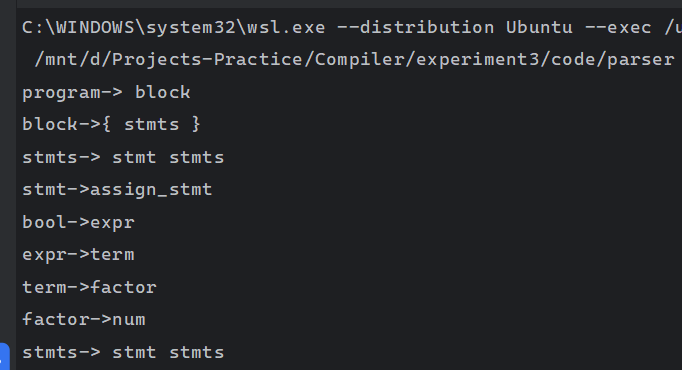
\includegraphics[width=0.6\linewidth]{output.png}
	\caption{运行结果}
	\label{fig:output}
\end{figure}


\section{Pratt Parser: 比LL(1)更优雅、同等高效地处理表达式}

Pratt Parser也被称为“优先表达式分析”(Precedence Parsing)。这种算法由美国计算机科学家Vaughan Pratt于1973年提出,
在JSLint这一著名的JavaScript语法检查工具中得到了应用。

Pratt Parser对于操作符的优先级和结合性进行处理,通过定义不同的优先级和绑定(左结合、右结合等)来处理表达式。
这种算法可以被认为是一种自顶向下的分析方法,与传统的LL(1)和LR(1)方法类似,但具有更好的灵活性和适应性。

与基于BNF语法来决定动作的LL(k)不同,Pratt Parser是基于Token的种类根据优先级和结合性来决定动作的。
这种方法的优点是,在很容易地处理操作符的优先级和结合性的同时,最大限度地避免回溯,因而比自顶向下的分析更为高效。
例如考察要求中给定的文法中的表达式部分:
\inputminted{bnf}{text/grammar.txt}
假设给定一个简单的单变量赋值语句$a=b;$,为了分析右侧的变量表达式$b$,普通的自顶向下分析需要依次调用
\texttt{bool}、\texttt{expr}、\texttt{term},\texttt{factor},才能选定给定的输入串$b$对应的产生式\texttt{factor -> id}。
在这一个例子中,给定的表达式仅仅造成了4次函数调用,但是在实际的编程语言中,表达式的复杂性往往会造成更多的函数调用,在一个递归过程中,
更多的函数调用会造成更多的栈空间的使用,从而造成更多的内存开销,也限制了表达式的处理深度。

产生这一现象的原因在于,为了让文法能够有效表达优先级和结合性,并且消除左递归,BNF文法被大大复杂化了。而普通的自顶向下分析,或者
LL(1)预测分析都依赖于文法决定分析动作,因此这是无法避免的。

在其论文中\emph{Top Down Operator Precedence},Vaughan Pratt详细描述了这一现象:
\begin{quotation}
The traditional mechanism for assigning meanings to programs is to associate semantic rules with phrase-structure rules, or equivalently, with classes of phrases. This is inconsistent with the following reasonable model of a programmer.

The programmer has in mind a set of semantic objects. His natural inclination is to talk about them by assigning them names, or tokens. He then makes up programs using these tokens, together with other tokens useful for program control, and some purely syntactic tokens. (No clear-cut boundary separates these classes.) This suggests that it is more natural to associate semantics with tokens than with classes of phrases.
\end{quotation}
当程序员写程序时,与普通的自顶向下分析器不同,他们并非根据语法规则决定语义进而构造程序,而是将语义对象赋予名字,然后他们就成为了代码中的Token。
这样一来,根据Token的种类来决定语义动作就成为了一种更为自然的方法。

并且在其论文中也提到了LL(k)分析的缺陷,这些缺陷也跟我实现真实世界中的编译器\footnote{开源在GitHub上:\url{https://github.com/SmartPolarBear/clox}}时的经验相吻合:
\begin{quotation}
A number of down-to-earth issues are not satisfactorily addressed by their system – deficiencies which we propose to make up in the approach below; they are as follows.

From the point of view of the language designer, implementer or extender, writing an LL(k) grammar, and keeping it LL(k) after extending it, seems to be a black art, whose main redeeming feature is that the life-support system can at least localize the problems with a given grammar. It would seem preferable, where possible, to make it easier for the user to write acceptable grammars on the first try, a property of the approach to be presented here.

There is no "escape clause" for dealing with non-standard syntactic problems (e.g. Fortran format statements). The procedural approach of this paper makes it possible for the user to deal with difficult problems in the same language he uses for routine tasks.

The life-support system must be up, running and debugged on the user's computer before he can start to take advantage of the technique. This may take more effort than is justifiable for one-shot applications. We suggest an approach that requires only a few lines of code for supporting software.

Lewis and Stearns consider only translators, in the context of their LL(k) system; it remains to be determined how effectively they can deal with interpreters. The approach below is ideally suited for interpreters, whether written in software, firmware or hardware.
\end{quotation}
这包括:不易于扩展、无法处理上下文无关文法无法处理的问题(例如Python中的缩进,以及原文提到的Fortran格式化语句)、需要大量的辅助代码等。

因此,在我的实现中,虽然输出结果和自顶向下分析的语法定义保持了一致,但是实际分析过程中,对于表达式,我使用Pratt Prasing进行了实现。

它需要为标志着表达式的Token定义下面的内容:
\begin{itemize}
	\item 优先级
	\item 在整个表达式中作为表达式前缀的处理函数
	\item 在整个表达式中作为表达式中缀的处理函数
\end{itemize}

然后,直接使用优先级就可以驱动分析过程,而不必依赖于文法。

例如,在我的实现中定义了代码~\ref{code:prec}的优先级和结合性规则。
\begin{listing}[htb]
	\caption{优先级和结合性规则表}
	\label{code:prec}
	\begin{minted}{cpp}
	std::unordered_map<token_type, rule> expr_rules{
		{token_type::TK_LPAREN, rule{PREC_NONE, &parser::grouping, nullptr}},
		{token_type::TK_PLUS, rule{PREC_TERM, &parser::unary, &parser::binary}},
		{token_type::TK_MINUS, rule{PREC_TERM, &parser::unary, &parser::binary}},
		{token_type::TK_DIVIDE, rule{PREC_FACTOR, nullptr, &parser::binary}},
		{token_type::TK_MULTIPLY, rule{PREC_FACTOR, nullptr, &parser::binary}},
		{token_type::TK_NEQ,rule{PREC_EQUALITY, nullptr, &parser::binary}},
		{token_type::TK_EQ,rule{PREC_EQUALITY, nullptr, &parser::binary}},
		{token_type::TK_GT,rule{PREC_COMPARISON, nullptr, &parser::binary}},
		{token_type::TK_GTE,rule{PREC_COMPARISON, nullptr, &parser::binary}},
		{token_type::TK_LT,rule{PREC_COMPARISON, nullptr, &parser::binary}},
		{token_type::TK_LTE,rule{PREC_COMPARISON, nullptr, &parser::binary}},
		{token_type::TK_NUM, rule{PREC_NONE, &parser::unary, nullptr}},
		{token_type::TK_ID, rule{PREC_NONE, &parser::unary, nullptr}},
	};
	\end{minted}
\end{listing}
而Pratt Parsing的驱动程序如代码~\ref{code:pratt}。首先根据当前Token选择
前缀规则,然后向右侧继续选择中缀规则,直到遇到优先级低于当前优先级的Token。
从代码中易见得,为了分析前述的例子中的$b$,仅需要一次函数调用即可完成。这大大
提高了效率。

需要注意的是,这种方式虽然和LL(1)分析达到了近乎一致的效果,但它在工程上的优势是显著的:

真实世界中的语言对优先级、结合性的是相当复杂的,为此构建文法、消除左递归、建立分析表的过程
将会相当复杂,这导致深层嵌套的语法,还有难以保证文法预处理正确的问题。而Pratt Parsing则只需要
这是因为在LL(1)分析中,我们需要将这些信息隐式地编码在文法中,而Pratt Parsing则将这些信息显式地
编码在了分析表中,这使得我们可以更加直观地理解和修改这些信息。这带来了极大的工程上的优势

\begin{listing}[htb]
	\caption{Pratt Parsing}
	\label{code:pratt}
	\begin{minted}{cpp}
// pratt parsing
void parser::all_expr(precedence prec)
{
	// Get the next token
	auto token = advance();

	// Get the prefix parse function for the token
	auto prefix = expr_rules[token->type].prefix;

	// Check if there is a prefix parse function for the token
	if (!prefix)
	{
		throw std::runtime_error("Unexpected token: " + token->lexeme);
	}

	// Parse the prefix expression
	auto left = (this->*prefix)();

	// Loop until the precedence is lower than the current precedence
	while (prec <= expr_rules[peek()->type].pred)
	{
		// Get the infix parse function for the next token
		auto in_tk = advance();
		auto infix = expr_rules[in_tk->type].infix;

		// Parse the infix expression
		left = (this->*infix)(left);
	}

	// Return the parsed expression
//	return left;
}
	\end{minted}
\end{listing}


\clearpage
\appendix
\section{附录:完整输出}
\label{sec:fullout}

\inputminted{bnf}{text/output.txt}

\end{spacing}

\end{document}